\documentclass{article}

% Chinese Support using xeCJK
% \usepackage{xeCJK}
%\setCJKmainfont{SimSun}

% Chinese Support using CTeX
% \usepackage{ctex}

% Math Support
\usepackage{amsmath}
\usepackage{amsfonts}
\usepackage{amssymb}
\usepackage{wasysym}
\newcommand{\angstrom}{\text{\normalfont\AA}}

% Graphics Support
\usepackage{graphicx}
\usepackage{float}

% Reduced page margin
\usepackage{geometry}
\geometry{a4paper,scale=0.8}

\usepackage{caption}
\usepackage{subcaption}

% d and e should be math operators
\newcommand*{\dif}{\mathop{}\!\mathrm{d}}
\newcommand*{\md}{\mathop{}\!\mathrm{d}}
\newcommand*{\me}{\mathrm{e}}

% No indent for each paragraph
\usepackage{parskip}
\setlength{\parindent}{0cm}

% Bold style for Greek letters
\usepackage{bm}
\let\Oldmathbf\mathbf
\renewcommand{\mathbf}[1]{\boldsymbol{\Oldmathbf{#1}}}

% More space for dfrac in cell
\usepackage{cellspace}
\setlength{\cellspacetoplimit}{5pt}
\setlength{\cellspacebottomlimit}{5pt}

% SI units
\newcommand{\si}[1]{\  \mathrm{#1}}

% Multi-line author information
\usepackage{authblk}
\author{Xiping Hu}
\affil{https://hxp.plus/}

\title{Homework for Chapter 9}

\begin{document}

\maketitle

\begin{figure}[H]
  \centering
  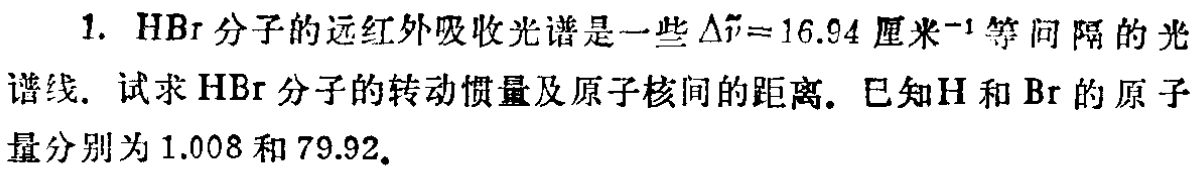
\includegraphics[width=\linewidth]{figures/Problem1}
  \label{fig:}
\end{figure}

\begin{equation*}
  \left\{
    \begin{aligned}
      & \Delta \tilde{\nu} = 2 B \\
      & B = \dfrac{h}{8 \pi^2 I c} \\
      & \mu = \dfrac{m_1 m_2}{m_1 + m_2} \\
      & I = \mu r^2
    \end{aligned}
  \right.
  \quad \Rightarrow \quad
  \left\{
    \begin{aligned}
      & I = 3.302 \times 10^{-47} \si{kg \cdot m^2} \\
      & r = 1.42 \si{\angstrom}
    \end{aligned}
  \right.
\end{equation*}

\begin{figure}[H]
  \centering
  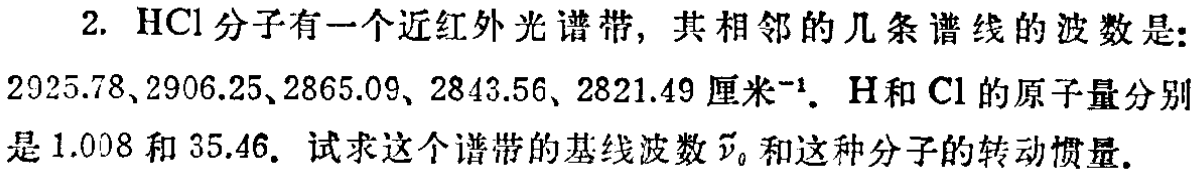
\includegraphics[width=\linewidth]{figures/Problem2}
  \label{fig:}
\end{figure}

\begin{equation*}
  \left\{
    \begin{aligned}
      \tilde{\nu}_{R1} = \tilde{\nu}_0 + 2 B = 2906.25 \si{cm^{-1}} \\
      \tilde{\nu}_{P1} = \tilde{\nu}_0 - 2 B = 2865.09 \si{cm^{-1}} \\
      \tilde{\nu}_{R2} = \tilde{\nu}_0 + 4 B = 2925.78 \si{cm^{-1}} \\
      \tilde{\nu}_{P2} = \tilde{\nu}_0 - 4 B = 2843.56 \si{cm^{-1}}
    \end{aligned}
  \right.
  \quad \Rightarrow \quad 
  \begin{aligned}
    \bar{B} = \dfrac{1}{2} \left( \dfrac{\tilde{\nu}_{R1} - \tilde{\nu}_{R2}}{4} + \dfrac{\tilde{\nu}_{R2} - \tilde{\nu}_{P2}}{8}  \right) = 10.285 \si{cm^{-1}} 
  \end{aligned}
\end{equation*}

\begin{equation*}
  \Rightarrow \quad
  \left\{
    \begin{aligned}
      & I = \dfrac{h}{8 \pi^2 B c} = 2.72 \times 10^{-47} \si{kg \cdot m^2} \\
      & \tilde{\nu}_0 = \dfrac{\tilde{\nu}_{R1} + \tilde{\nu}_{R2} +\tilde{\nu}_{P1} +\tilde{\nu}_{P2}}{4} = 2885.17 \si{cm^{-1}}
    \end{aligned}
  \right.
\end{equation*}

\begin{figure}[H]
  \centering
  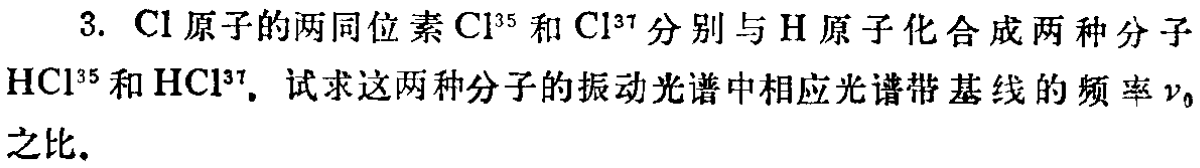
\includegraphics[width=\linewidth]{figures/Problem3}
  \label{fig:}
\end{figure}

\begin{equation*}
  \begin{aligned}
    \tilde{\nu} = \dfrac{1}{2 \pi c} \sqrt{\dfrac{k}{m} } 
  \end{aligned}
  \quad \Rightarrow \quad 
  \begin{aligned}
    \dfrac{\tilde{\nu}_{01}}{\tilde{\nu}_{02}} = \sqrt{\dfrac{m_2}{m_1} } = 1.002
  \end{aligned}
\end{equation*}

\begin{figure}[H]
  \centering
  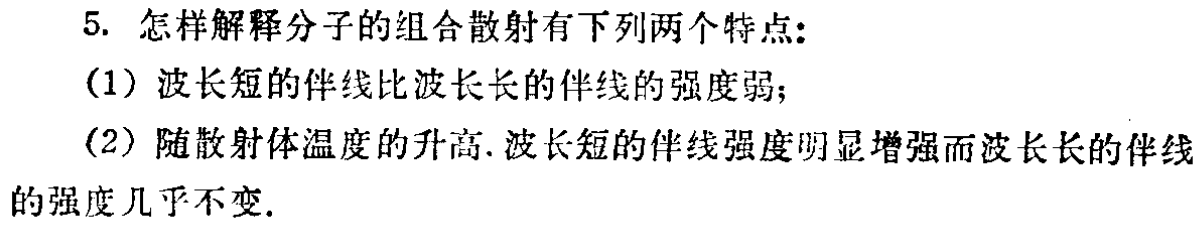
\includegraphics[width=\linewidth]{figures/Problem5}
  \label{fig:}
\end{figure}

According to statistics regulations, molecules tend to stay on low energy levels, thus the amount of molecules on high energy levels is far more smaller than the amount of molecules an low energy levels. So that the majority of molecules will emit light with long wavelength, while few molecules emit light with short wavelength. This causes the irradiance of light with short wavelength lower than those with long wavelength.

But when the temperature becomes higher, according to Boltzmann Statistics, more molecules will exist in high energy levels, thus the irradiance of light with short wavelength will become higher.

\end{document}